\documentclass[11pt]{beamer}
%\usetheme[faculty=fi,nofonts]{fibeamer}
\usetheme[
  workplace=fi,
]{MU}

\usepackage[utf8]{inputenc}
\usepackage[czech]{babel}
\usepackage[T1]{fontenc}
\usepackage{amsmath}
\usepackage{amsfonts}
\usepackage{amssymb}
\usepackage{amsthm}
\usepackage{graphicx}
\usepackage{listings}
\usepackage[margin=1.5cm]{caption}
\usepackage{float}

\author{Jan Tušil}
\title{Angelic Verification}
\subtitle{Precise Verification Modulo Unknowns}
%\setbeamercovered{transparent} 
%\setbeamertemplate{navigation symbols}{} 
%\logo{} 
%\institute{} 
%\date{2018-03-23} 
%\date{2018-03-23} 
%\subject{} 

\newtheorem{dfn}{Definice}

%\floatstyle{boxed} 
%\restylefloat{figure}

%\floatstyle{boxed}
%\newfloat{program}{thp}{lop}
%\floatname{program}{Program}

\lstset{
basicstyle=\footnotesize\ttfamily,
%numbers=left, 
%numberstyle=\small, 
%numbersep=4pt, 
%frame = single, 
%language=Pascal, 
%framexleftmargin=15pt
}

\begin{document}

% Ahoj,
% dneska se budeme věnovat článku zvaném "Angelic Verification: Precise
% Verification Modulo Unknowns", který vyšel na CAVu v roce 2015.
% Myšlenky z tohoto článku byly implementovány v nástroji
% AngelicVerifier, a autoři (z Microsoftu) tvrdí, že je tento nástroj může soutěžit
% s nástroji SDV a PREfix, ovšem s výrazně nižšími nároky na práci uživatele.
\begin{frame}
\titlepage
\end{frame}

% Jak na začátek?
% V programech mohou nastávat běhové chyby - třeba zápisy mimo hranice pole
% nebo selhání uživatelských assertů. Máme-li program P, můžeme se ptát:
% existuje běh programu P, v němž dojde k selhání assertu?
% Tato otázka je ještě složitější, pokud nemáme jasno v tom, jaké iniciální stavy uvažujeme
% a co dělají některé části programu - třeba volání systému nebo knihoven, od nichž nemáme k dispozici zdrojový kód.


% Uvažujme například tento program:
% Máme zde pole m a vstupním bodem je zde funkce Foo,
% která bere jako parametr hodnotu typu int.
% Tuto hodnotu ignoruje a volá funkci Baz,
% které svůj parametr použije jako index do pole.
% Pokud y je NULL, dojde k chybě. V tomto programu je bug,
% na 100%.
\begin{frame}[fragile]{Příklad}
\begin{semiverbatim}
\textbf{var} m:[\textbf{int}]\textbf{int};
\pause
// entry point
\textbf{procedure} Foo(z:\textbf{int}) \{
  \textbf{call} Baz(NULL);
\}
\pause
\textbf{procedure} Baz(y:\textbf{int}) \{
  \textbf{assert} y != NULL; \uncover<4->{// 100\% bug}
  m[y] := 4;
\}
\end{semiverbatim}
\end{frame}


% Uvažme jiný program.
% Máme zde obět pole m a ještě jednu proměnnou.
% Procedura Foo obět bere parametr, ale tentokrát ho
% předává proceduře Bar. V té je ale chyba.
% Nebo není? Co kdybychom řekli, že Foo nesmí brát jako parametr null?
% Pak by ale byl kus kódu v Bar nedosažitelný.
\begin{frame}[fragile]{Jiný příklad}
\begin{semiverbatim}
\textbf{var} gs:\textbf{int}, m:[\textbf{int}]\textbf{int};
\pause\only<5->{// precondition: z != NULL}
// entry point
\textbf{procedure} Foo(z:\textbf{int}) \{
  \textbf{call} Bar(z);
\}\pause
\uncover<8->{// inconsistent}
\textbf{procedure} Bar(x:\textbf{int}) \{
  \textbf{if} (x != NULL) \{ gs := 1;\only<7->{ // unreachable} \}
  \textbf{else} \{ gs := 2; \}
  \textbf{assert} x != NULL; \only<4-5>{// bug}\only<6->{// ok due to precondition}
  m[x] := 5;
\}
\end{semiverbatim}
\end{frame}


% Třetí příklad. Opět máme globální pole,
% a navíc dvě knihovní funkce, jejichž implementaci neznáme.
% Procedura Foo je opět vstupním bodem programu, a tentokrát
% volá procedu FooBar, ignorujíc přitom svůj parametr.
% <Popis FooBar>
% Může dojít k selhání assertu?
\begin{frame}[fragile]{Do třetice \ldots}
\begin{columns}

\begin{column}{0.5\textwidth}
\begin{semiverbatim}
\textbf{var} m:[\textbf{int}]\textbf{int};
\pause
// library
\textbf{procedure} Lib1() \{
  \textbf{returns} (r:\textbf{int})\only<-6>{;}
  \only<7->{\textbf{ensures} (r != NULL);}
\textbf{procedure} Lib2()
  \textbf{returns} (r:\textbf{int})\only<-10>{;}
  \only<11->{\textbf{ensures} (r != NULL);}
\pause
// entry point
\textbf{procedure} Foo(z:\textbf{int}) \{
  \textbf{call} FooBar();
\}
\end{semiverbatim}
\end{column}

\begin{column}{0.5\textwidth}
\begin{semiverbatim}
\uncover<14->{\textbf{allways} Lib1() != Lib2();}
\pause
\textbf{procedure} FooBar() \{
  \textbf{var} x, w, z:\textbf{int}\pause\onslide<+->
  \textbf{call} z := Lib1();\onslide<+->
  \textbf{assert} z != NULL;\pause\onslide<+->
  m[z] := NULL;\onslide<+->
  \textbf{call} x := Lib2();\onslide<+->
  \textbf{assert} x != NULL;\pause\onslide<+->
  w := m[x];\onslide<+->
  \textbf{assert} w != NULL;\pause\onslide<+->
  m[w] := 4;\onslide<4->
\}
\end{semiverbatim}
\end{column}

\end{columns}
\end{frame}

\begin{frame}{Shrnutí}

\end{frame}

%=======================================================================================
% Otevřené a uzavřené programy, plané poplachy
% Začněme příkladem.

% Řekněme, že máme nástroj, kterému předhodíme program a on nám řekne,
% jestli existuje běh tohoto programu z nějakého iniciálního stavu
%\begin{frame}[fragile]{Uzavřené vs otevřené programy}
%
%
%\end{frame}
%
%% Zabýváme se hledáním běhových chyb či prokazováním jejich absence.
%% Chyby jsou modelovány selhanými asserty.
%
%% Hmm... ta otevřenost může způsobit plané poplachy,
%% které jsou plané v tom smyslu, že předpokládají nějaké použití programu,
%% které v reálu nenastane - třeba proto, že ten program pro něj není urrčený.
%
%
%% Uvažme například tento program v jazyce Boogie,
%% který vznikl zakletím nějakého programu z jazyka C.
%% Přičemž ukazatele jsou zde modelovány jako čísla, která jsou následně
%% použitá pro indexování pole m.
%
%% Za vstupní bod považujme proceduru Foo.
%% Hmm... nebo klidne vsechny
%
%% Jaké jsou zde zdroje neznámých, neomezených hodnot?
%% (Parametr z, procedury Lib1, Lib2).
%% Které z těchto assertů mohou selhat?
%% Ve vší obecnosti, pokud o neznámých hodnotách nic nepředpokládáme,
%% mohou selhat všechny. Přesto, když programátor dostane
%% od nástroje pět varování, nebude z nich úplně nadšený
%% - on přece ví, že funkce Lib2 nevrací NULL.
%% Bylo by fajn tahle varování nějak seřadit,
%% třeba podle toho, jak jsou užitečná.
%
%% Chya určitě při volání baz. Nejspíš ano v bar - nekonzistence.
%% Asi ne pro FooBar. Je celkem rozumné předpokládat, že daná knihovní funkce nevrací NULL.
%\begin{frame}{Otevřený program - příklad}
%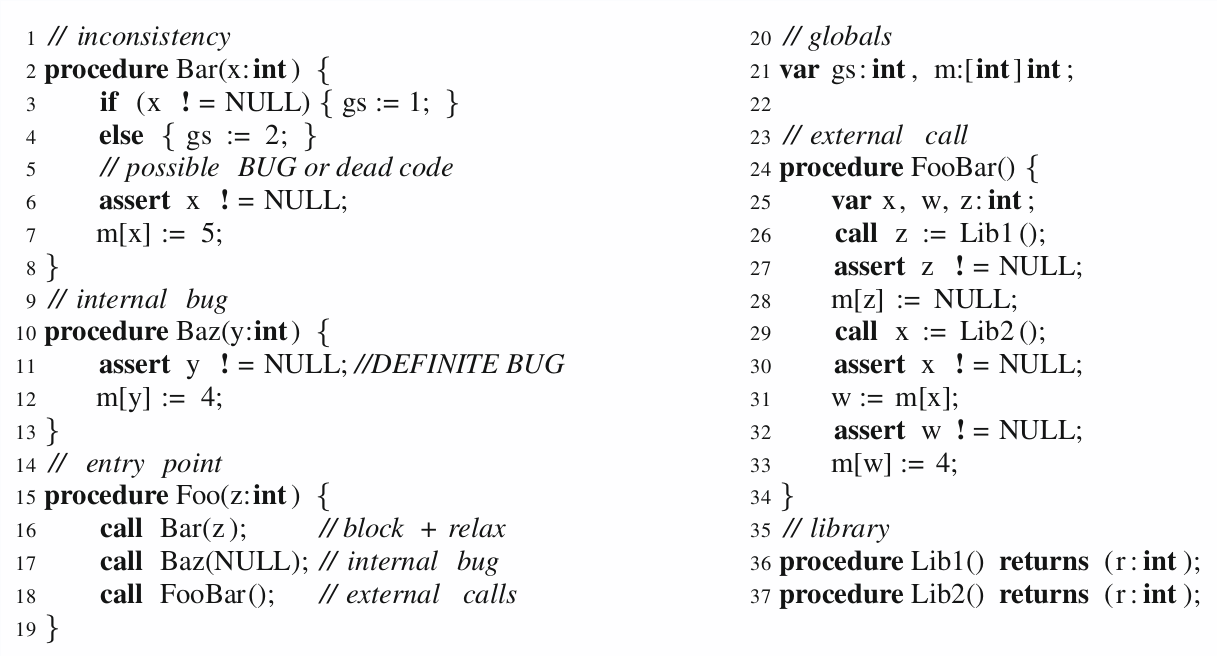
\includegraphics[width=1.0\linewidth]{img/exampleProgram.png}
%\end{frame}
%%
%%\begin{frame}[fragile]{Některé stopy programu}
%%\begin{lstlisting}
%%push; // call bar
%%gs := 2;
%%assert x != null;
%%fail;
%%\end{lstlisting}
%%\end{frame}
%%
%%\begin{frame}[fragile]
%%\begin{lstlisting}
%%int gs;
%%void bar(int *x) {
%%  if (x != nullptr) gs = 1;
%%  else gs = 2;
%%  *x = 5;
%%}
%%
%%void baz(int *y) {
%%  *y = 4;
%%}
%%
%%void foo(int *z) {
%%  bar(z);
%%  baz(nullptr);
%%}
%%
%%int ** Lib1();
%%int ** Lib2();
%%void FooBar() {
%%  *Lib1() = NULL;
%%  **Lib2() = 4;
%%}
%%\end{lstlisting}
%%\end{frame}
%
%
%\begin{frame}{Cíl}
%\begin{itemize}
%\item cíl: prioritizace důležitějších alarmů
%\item  metoda: angelická verifikace (i.e. abduktivní inference)
%\end{itemize}
%
%\begin{dfn}[Problém angelické verifikace]
%Pro daný assert, existuje přijatelná specifikace nad neznámými hodnotami taková,
%že daný assert platí?
%\end{dfn}
%
%Chceme, aby přijatelná specifikace byla:
%\begin{itemize}
%\item stručná
%\item shovívavá
%\end{itemize}
%
%\end{frame}
%
%\section{Detaily}
%
%% Uvažujme jednoduchý jazyk (který je prý podmnožinou jazyka Boogie).
%% Program je tvořen posloupností základních bloků,
%% přičemž blok se skládá z posloupnosti příkazů a je ukončen
%% seznamem následných bloků.
%\begin{frame}{Jazyk}
%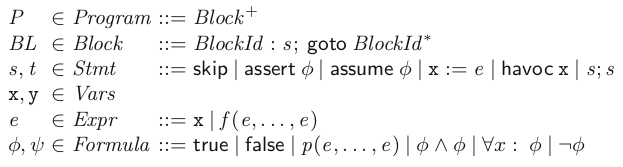
\includegraphics[width=0.9\linewidth]{img/boogieSubset.png}
%\end{frame}
%
%% Uvažujeme běhovou sémantiku, tj. každému programu přiřazujeme
%% množinu běhů, což jsou konečné i nekonečné posloupnosti
%% stavů. Stav je přitom jen valuace proměnných.
%
%% Teď tu neřešíme pole.
%\begin{frame}{Sémantika}
%\begin{itemize}
%\pause \item stavy: $\Sigma = \left( \textsc{Valuace proměnných} \right) \cup \{ \textit{Err} \} $
%%\pause \item stavy: $\Sigma = \left(\textit{Vars} \rightarrow \mathcal{Z} \right) \cup \{ \textit{Err} \} $
%\pause \item běhy: $\textit{Traces} = \Sigma^* \cup \Sigma^\omega$
%\pause \item Sémantika $\mathcal{T} = \textit{Program} \rightarrow \mathcal{P}(\textit{Traces})$ dle očekávání
%\pause \item selhaný \lstinline|assert(E)| - běh obsahuje stav $\textit{Err}^\omega$
%\pause \item selhaný \lstinline|assume(E)| - běh je neuskutečnitelný
%\end{itemize}
%
%\pause 
%
%\begin{dfn}
%Program $P$ je korektní, píšeme $\vDash P$, pokud $\mathcal{T}(P)$ neobsahuje stopu obsahující stav $\textit{Err}$.
%\end{dfn}
%\end{frame}
%
%% V tomto jazyce nejsou řídící podmínky, jen goto.
%% Přesto je možné psát v něm programy.
%% Ukázka kódu v tonto jazyce.
%% Idea: běhy, v nichž nastane assume(false), nás nezajímavjí.
%% Tedy... nekonečné nechybové běhy nás nezajímají.
%% Tedy, v tomto jazyku můžeme modelovat i řídící struktury.
%\begin{frame}[fragile]{Ukázka}
%\begin{columns}
%
%\begin{column}{0.5\textwidth}
%Co počítá tento program?
%\uncover<2->{Jak vypadají uskutečnitelné běhy?}
%\begin{lstlisting}
%start:
%  sum := 0;
%  i := n; 
%  goto cycle end
%    
%cycle:
%  assume i > 0;
%  sum *= i;
%  i--;
%  goto cycle end
%  
%end:
%  assume i <= 0;
%  goto
%\end{lstlisting}
%\end{column}
%
%\begin{column}{0.5\textwidth}
%\pause \pause
%Řídící struktury: kód ve tvaru
%%\begin{semiverbatim}
%%if (E) { S } else { T }
%%\end{semiverbatim}
%\begin{lstlisting}
%if (E) { S } else { T }
%\end{lstlisting}
%lze přepsat jako
%\begin{lstlisting}
%Start: goto Then, Else
%Then: assume E; S; goto End
%Else: assume !E; T; goto End
%End: /* ... */
%\end{lstlisting}
%\end{column}
%\end{columns}
%\end{frame}
%
%% Teď už máme sémantiku jazyka, a můžeme definovat vstupní podmínku
%\begin{frame}[fragile]{Korektnost se vstupní podmínkou}
%\begin{dfn}
%Program $P \in \textit{Program}$ je korektní se vstupní podmínkou $\phi \in \textit{Formula}$,
%píšeme $\phi \vDash P$, pokud je korektní program:
%\begin{lstlisting}
%Start0 : assume phi; goto Start
%\end{lstlisting}
%\end{dfn}
%
%\pause
%
%% Kromě obyčejných assertů již přítomných v programu
%% budeme pracovat i s uživatelem přidanými andělskými asserty.
%% Jak uvidíme, tyto budou sloužit k vyjádření toho, co považujeme
%% za rozumnou vstupní podmínku.
%% Oba druhy assertů však mají stejnou sémantiku v našem programovacím jazyce.
%% Tato definice nám jen umožňuje přidávat a odebírat asserty do programu.
%\begin{dfn}
%Nechť $A$ je množina obyčejných assertů v programu $P$,
%a nechť $\hat{A}$ je množina andělských assertů 
%uživatelem přidaných do programu $P$. Výrazem $P_{A_1, A_2}$
%označujeme instrumentovanou verzi programu $P$ ,
%která má povolené pouze
%%obyčejné
%asserty $A_1 \subseteq A$
%a
%%andělské asserty
%$A_2 \subseteq \hat{A}$.
%\end{dfn}
%
%\end{frame}
%
%% Chceme nějak vyjádřit, že vstupní podmínka není moc přísná.
%% Například pod vstupní podmínkou false je každý program korektní.
%% Pomocí andělských assertů, které nám poskytne uživatel,
%%  tedy definujeme shovívavou vstupní podmínku.
%\begin{frame}{Shovívavá vstupní podmínka}
%\begin{dfn}[Shovívavá vstupní podmínka]
%Formule $\phi$ je shovívavá vstupní podmínka programu $P_{A, \hat{A}}$,
%značíme $Permissive\left( P_{A, \hat{A}}, \Phi \right)$,
%pokud pro každý andělský assert $s \in \hat{A} $ platí:
%pokud $\phi \vDash P_{\emptyset, \{ s \} }$, pak  $\textsc{true} \vDash P_{\emptyset, \{ s \} } $.
%\end{dfn}
%
%\pause Jak to říci jinak?
%
%\pause Jak vypadají shovívavé vstupní podmínky programu, který obsahuje andělský
%\begin{itemize}
%\pause \item \lstinline|assert false| na začátku programu?
%\pause \item \lstinline|assert false| na konci každého bloku?
%\pause \item \lstinline|assert x != v| někde?
%\end{itemize}
%
%\end{frame}
%
%% Pomocí shovívavých vstupních podmínek definujeme andělskou korektnost.
%\begin{frame}{Andělská korektnost}
%\begin{dfn}
%Mějme program P obsahující sadu běžných assertů $A$
%a sadu andělských assertů $\hat{A}$, spolu se slovníkem formulí \texttt{Vocab}.
%Říkáme, že P je andělsky korektní za předpokladu $( \texttt{Vocab}, \hat{A} )$,
%pokud existuje formule $\phi \in \textsf{Vocab}$, která je shovívavou vstupní podmínkou programu P,
%a přitom $\phi \vDash P_{A, \emptyset}$. 
%\end{dfn}
%\end{frame}
%
%% Předpokládejme teď, že Vocab je množina všech formulí.
%% a andělská asserty jsou právě asserty uvedené modře.
%% Je tento program andělsky korektní? S jakým předpokladem?
%% Možné podmínky: false, x > 100
%\begin{frame}[fragile]{Je andělsky korektní?}
%Obyčejné asserty černě, andělské asserty \textcolor{blue}{modře}.
%%\setbeamerfont{alerted text}{series=\footnotesize,family=\ttfamily}
%\begin{semiverbatim} \small
%start:
%  \only<2>{\textcolor{blue}{assert x > 5;}}\only<3>{\textcolor{blue}{assert x > 2;}}
%  assert x > 3;
%  goto
%\end{semiverbatim}
%
%
%\end{frame}
%
%% Mějme takovýto kód.
%\begin{frame}[fragile]{Příklad}
%\begin{semiverbatim} \small
%start:
%  \uncover<4->{\textcolor{blue}{assert m1 != m2}}
%  goto L1 L2
%L1:
%  assert !locked(m1); lock(m1); goto
%L2:
%  assert locked(m2); unlock(m2); goto
%\end{semiverbatim}
%\uncover<2->{Možná precondition: $m1 \not = m2$.}
%\uncover<3->{Ale co když uživatel ví, že někdy $m1 = m2$?}
%\uncover<5->{Nyní již specifikace $m1 \not = m2$ nemusí být shovívavá.}
%\end{frame}
%
%% Předpokládejme, že máme funkci Verify, které můžeme předhodit
%% program a vstupní podmínku. Tato funkce rozhodne,
%% jestli každý z běhů, jejichž iniciální stav splňuje vstupní podmínku,
%% naplní asserty. Pokud ne, vrátí takovýto běh.
%
%% Algoritmus pro angelickou verifikaci funguje tak,
%% že začíná s prázdnou specifikací (tj. true), 
%% a postupně ji zjemňuje tak dlouho,
%% dokud v programu stále existuje chybový běh.
%% Z tohoto chybového běhu se vyextrahuje formule,
%% která tento běh blokuje, a přidá se do specifikace.
%
%% Může se ale stát, že takovou formuli nebudeme schopni najít,
%% nebo bude vzniklá specifikace příliš tvrdá (nebude shovívavá)
%% - například nebude vůbec splnitelná. V takovém případě algoritmus novou formuli nepoužije
%% a odebere selhávající assert z množiny assertů, které se snaží dokázat.
%\begin{frame}{AngelicVerifier}
%\begin{columns}
%
%\begin{column}{0.5\textwidth}
%Algoritmus rozhodující andělskou korektnost.
%\begin{itemize}
%\pause \item Vstupy: program $P$ s obyčejnými asserty $A$ a andělskými asserty $\hat{A}$.
%\pause \item Výstupy: shovívavá specifikace $E$ a množina platících obyčejných assertů $A_1 \subseteq A$.
%\pause \item $\phi$ - formule blokující chybový běh $\tau$
%\end{itemize}
%\end{column}
%
%
%\begin{column}{0.5\textwidth}
%\pause 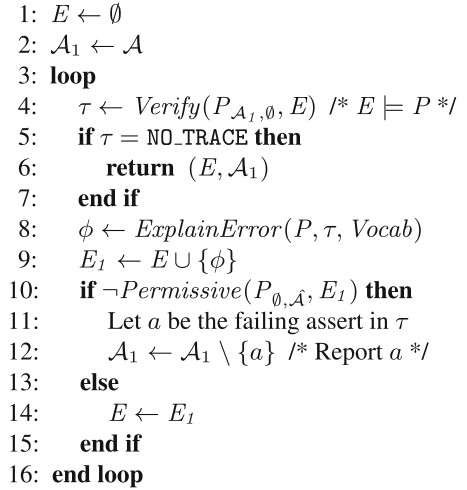
\includegraphics[width=0.9\linewidth]{img/angelicVerifyShort.png}
%\end{column}
%
%
%\end{columns}
%\end{frame}
%
%\begin{frame}{ExplainError}
%\begin{columns}
%
%% Vygeneruje bud formuli v CNF, nebo jen jednu klauzuli (ryhlejsi)
%\begin{column}{0.5\textwidth}
%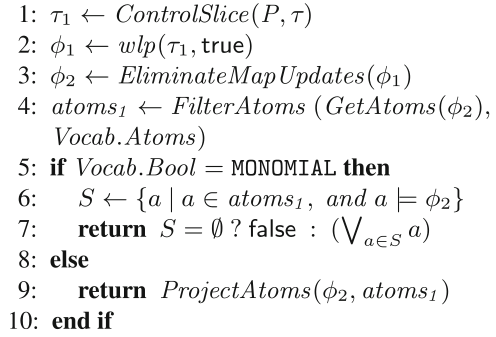
\includegraphics[width=0.9\linewidth]{img/explainErrorShort.png}
%\end{column}
%
%\begin{column}{0.5\textwidth}
%Explanation
%\end{column}
%
%\end{columns}
%\end{frame}
%
%% Říkám někde, že stopa je posloupnost příkazů?
%%\item stopa = program bez řídících struktur
%
%
%% Uvažme proceduru FooBar na obrázku.
%% Procedura Verify z algoritmu může vrátit třeba
%% takovoutu stopu tau, která porušuje poslední assert z FooBar.
%% Tuto stopu dostane ExplainError a zkusí z ní vytvořit
%% shovívavou vstupní podmínku, která tuto stopu zablokuje.
%\begin{frame}[fragile]{Příklad}
%\begin{columns}
%
%\begin{column}{0.5\textwidth}<1->
%%\begin{figure}
%%\frame{
%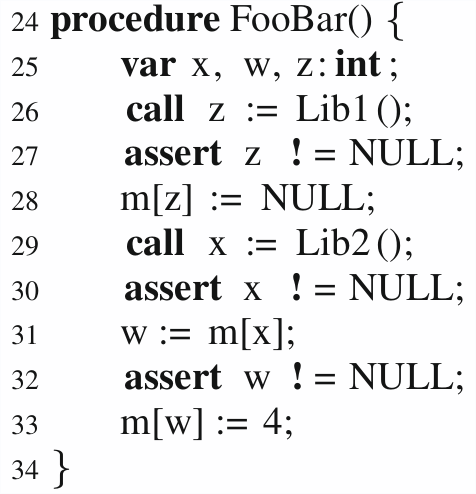
\includegraphics[width=0.9\textwidth]{img/fooBar.png}
%%}
%%\caption{Stopa se selhávajícím assertem.}
%%\end{figure}
%\end{column}
%
%\begin{column}{0.5\textwidth}<2>
%Stopa $\tau$:
%\begin{lstlisting}
%z := x_1;
%m[z] := NULL;
%x := x_2;
%w := m[x];
%assert w != NULL;
%\end{lstlisting}
%
%\begin{itemize}
%
%\item volání knihovních procedur nahrazena novými proměnnými
%\end{itemize}
%
%% $$wlp(\tau, true) = \textsc{read}(write(m, x_1, NULL), x_2) $$
%
%\end{column}
%
%\end{columns}
%\end{frame}
%
%
%% Klasický WP kalkulus s tím, že čtení a zápis
%% do polí modelujeme pomocí funkcí read a write.
%% Formule nad jazykem polí, arithmetiky, a rovností.
%% Zkusíme si to na tabuli sami spočítat
%\begin{frame}[fragile]{Příklad}
%%\begin{columns}
%
%%\begin{column}{0.5\textwidth}<1>
%Stopa $\tau$:
%\begin{lstlisting}
%z := x_1;
%m[z] := NULL;
%x := x_2;
%w := m[x];
%assert w != NULL;
%\end{lstlisting}
%
%\pause
%
%$wlp(\tau, true)$:
%\begin{lstlisting}
%read(write(m, x_1, NULL), x_2) != NULL
%\end{lstlisting}
%
%%\begin{lstlisting}
%%w != NULL
%%read(m, x) != NULL
%%read(m, x2) != NULL
%%read(write(m, z, NULL), x2) != NULL
%%read(write(m, x_1, NULL), x2) != NULL
%%read(write(m, x_1, NULL), x_2) != NULL
%%\end{lstlisting}
%
%\pause 
%
%EliminateMapUpdates:
%\begin{lstlisting}
%(x_2 == x_1 ? NULL : read(m, x_2)) != NULL
%x_1 != x_2 && read(m, x_2) != NULL
%\end{lstlisting}
%
%%\begin{lstlisting}
%%(x_2 == x_1 ? NULL : read(m, x_2)) != NULL
%%
%%(x_1 == x_2 -> NULL != NULL) && (x_1 != x_2 -> read(m, x_2) != NULL)
%%(x_1 == x_2 -> false) && (x_1 != x_2 -> read(m, x_2) != NULL)
%%(x_1 != x_2 || false) && (x_1 != x_2 -> read(m, x_2) != NULL)
%%(x_1 != x_2) && (x_1 != x_2 -> read(m, x_2) != NULL)
%%x_1 != x_2 && read(m, x_2) != NULL
%%\end{lstlisting}
%
%%\end{column}
%%\end{columns}
%\end{frame}
%
%\begin{frame}{Shrnutí}
%
%\end{frame}
%


\end{document}